\section{Mapserver}
MapServer adalah sebuah aplikasi freeware dan open source yang dapat menampilkan data spasial (peta) pada web. Aplikasi ini dikembangkan pertama kali oleh Universitas Minesotta, Amerika Serikat dalam projek ForNet yang merupakan sebuah projek untuk manajemen sumber daya alam yang disponsori NASA. kemudian dikembangkan projek TerraSIP sebagai manajemen data lahan. Karena sifatnya terbuka atau open source, pengembangan MapServer dilakukan oleh banyak negara.

\subsection{Cara Instalasi Mapserver}
\begin{enumerate}
\item
Download Mapserver atau disingkat MS4W di http://mapserver.org/download.html
\begin{figure}[ht]
	    \centerline{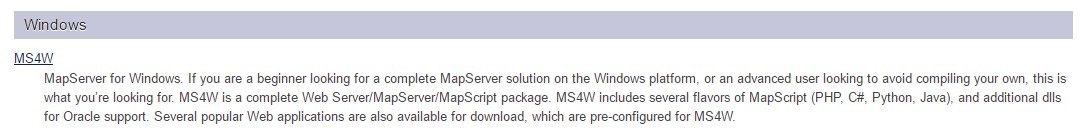
\includegraphics[width=0.50\textwidth]{figures/gambar1.JPG}}
	    \caption{Download MS4W}
		\label{gambar1}
		\end{figure}
\item
Setelah di download jalankan setupnya, disini saya menggunakan port 2000 karena port default 80 sudah dipakai oleh xampp
\begin{figure}[ht]
	    \centerline{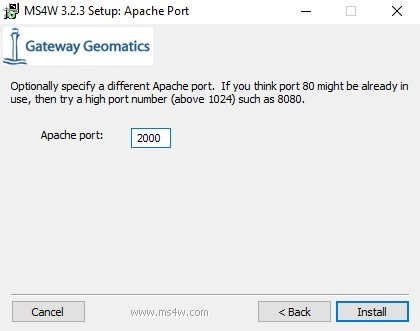
\includegraphics[width=0.50\textwidth]{figures/gambar2.JPG}}
	    \caption{Port 2000}
		\label{gambar2}
		\end{figure}
\item
Lalu tunggu instalasi sampai selesai
\begin{figure}[ht]
	    \centerline{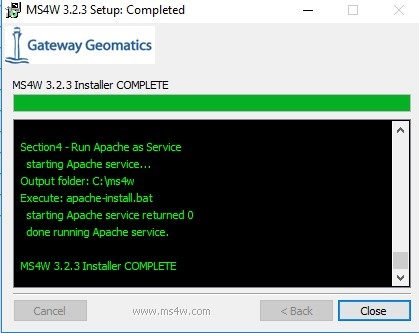
\includegraphics[width=0.50\textwidth]{figures/gambar3.JPG}}
	    \caption{Selesai}
		\label{gambar3}
		\end{figure}
\item
Setelah proses selesai silahkan buka browser favorit anda, kemudian ketikkan http://localhost:2000 di kotak isian URL.
\item
Jika anda melihat tampilan home MAPSERVER atau MS4W proses instalasi anda berhasil.
\begin{figure}[ht]
	    \centerline{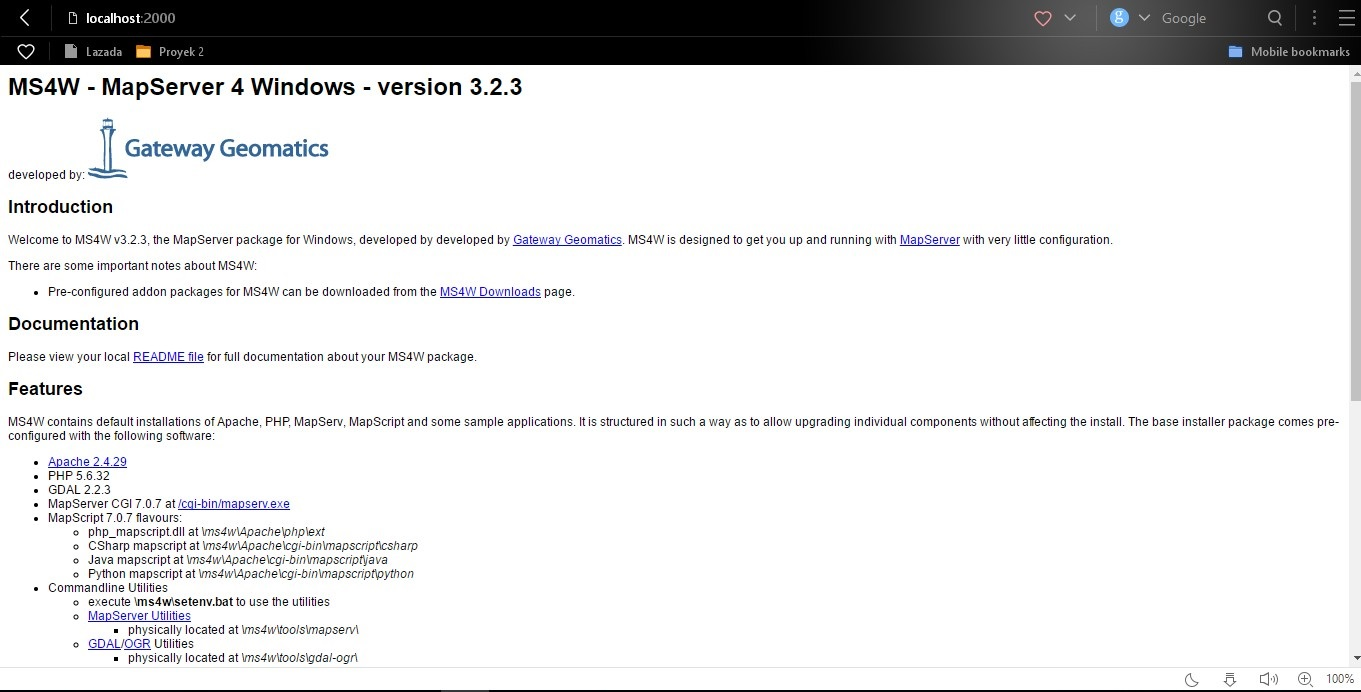
\includegraphics[width=0.50\textwidth]{figures/gambar4.JPG}}
	    \caption{Tampilan MS4W}
		\label{gambar4}
		\end{figure}
\end{enumerate}
